\documentclass[pdf,10pt,xcolor=dvipsnames,hide notes]{beamer}
\usetheme{boadilla}
\usecolortheme{seahorse} % or try albatross, beaver, crane, ...
\usepackage{verbatim}
%\usefonttheme{serif}     % Font theme: serif
\usepackage{ccfonts}     % Font family: Concrete Math
\usepackage[T1]{fontenc}
\usepackage{lmodern}
\usepackage{caption}
\usepackage[caption=false]{subfig}
\usepackage{tabularx}
\usepackage{booktabs}
\usepackage{pdfpages}
\usepackage{graphicx} 
\usepackage{hyperref}
\DeclareCaptionLabelSeparator{horse}{:\quad} % change according to your needs
\captionsetup{
  labelsep = horse,
  figureposition = bottom % proper spacing between figure and caption
}
\usepackage{graphicx,amsfonts,booktabs,hyperref,subfig,amssymb,amsmath,amsthm,tabularx,multirow,enumerate}
%\usepackage{parskip}
%\setlength{\parindent}{10pt}
\usepackage{ragged2e,tikz,color,colortbl,xcolor}

\DeclareMathOperator{\Ima}{Im}

% Real Number
\newtheorem{proposition}{Proposition}
\newcommand{\R}{\mathbb R}
% natural numbers
\newcommand{\Nat}{\mathbb N}
% complex numbers
\newcommand{\C}{\mathbb C}
\newcommand{\E}{\mathbb{E}}
\newcommand{\Var}{\mathrm{Var}}
\newcommand{\Cov}{\mathrm{Cov}}
\newcommand{\Corr}{\mathrm{Corr}}
\newcommand{\Expect}{{\rm I\kern-.3em E}}
\setbeamertemplate{theorems}[numbered]

\setbeamertemplate{caption}[numbered]
\setbeamercolor{postit}{use=structure,fg=black,bg=structure!13!white}
\newcommand{\otoprule}{\midrule[\heavyrulewidth]}
\makeatletter
    \newenvironment{withoutheadline}{
        \setbeamertemplate{headline}[default]
        \def\beamer@entrycode{\vspace*{-\headheight}}
    }{}
\makeatother
\title[\sc{XVIII EBFin}]{Robust Portfolio Optimization with Multivariate Copulas: A Worst-Case CVaR Approach}
\author[Sao Paulo/SP, July 20th]{\textbf{Fernando Sabino da Silva}\inst{1}, Flavio A. Ziegelmann\inst{1,2}}
\institute[]{\inst{1} Department of Statistics - UFRGS, \inst{2} Graduate Program in Economics - UFRGS}
%, Cristina Tessari\inst{3}, \inst{3} Finance Division - Columbia Business School
%\date{\today} % (optional)
\date{} % (optional)

\hypersetup{
    pdftitle={TITLE},
    pdfauthor={AUTHOR},
    pdfsubject={SUBJECT},
    pdfkeywords={KEYWORD} {KEYWORD} {KEYWORD},
    colorlinks=true,
    linkcolor=blue,
    citecolor=blue,
    filecolor=magenta,
    urlcolor=blue
    }
\usepackage{threeparttable}


\begin{document}
\justifying

\frame{\titlepage}

\section{Introduction}

\begin{frame}[label=frame1]
\frametitle{Introduction}

\begin{itemize}
\setlength{\parskip}{4pt}
\justifying

\item We address the uncertainty of the distribution of assets' returns in a CVaR minimization model by applying copula function and obtaining its robust counterpart

%\item Markowitz considered the problem of an agent who wishes to find the maximum (expected)
%return for a given level of risk or minimize risk for a given level of
%return.
\begin{itemize}
	\item Specifically, we obtain a numerical estimate of the worst Copula CVaR, where the copulas belong to the class of Archimedean copula, and evaluate its out-of-sample performance with Gaussian copula CVaR model and a constant mixed portfolio.
\end{itemize}

\end{itemize}

\end{frame}

\begin{frame}[label=frame1d]
\frametitle{Some Key Points}

\begin{itemize}
	 \setlength{\parskip}{15pt}
	\justifying
	\setbeamercovered{transparent}
	
	%		\item The original Markowitz model finds a set of "optimal" portfolio weights given
	%		a set of expected returns and covariances. 
	
\item<1> Worst-case copula conditional Value-at-Risk optimization using linear programming.
	
\item<2> Risk management with higher dimension than those typically considered in the copula literature without pair-copula constructions.
	
\item<3> We select a diversified set of assets that can be useful during any market conditions.
% i.e., that somehow involves hedging of decisionsto protect the investors against any market conditions
\end{itemize}

\end{frame}

\begin{frame}[label=frame1d]
	\frametitle{Background}
	
	\begin{itemize}
		 \setlength{\parskip}{15pt}
		\justifying
		\setbeamercovered{transparent}
		
		%		\item The original Markowitz model finds a set of "optimal" portfolio weights given
		%		a set of expected returns and covariances. 
		
	\item<1> A well-known problem of the Markowitz model is its sensitivity to the input parameters. 
		
	\item<1> This problem can be overcome by employing robust optimization and worst case techniques (\textcolor{blue}{Zhu and Fukushima}, \textcolor{blue}{2009}) in which assumptions about the distributions of the random variables are relaxed. 
	\setlength{\parskip}{0pt}
	\begin{itemize}
		\item Obtain the optimal portfolio solution by optimizing over a prescribed set and possible densities.
	\end{itemize}

\setlength{\parskip}{15pt}

\item<2>  \textcolor{blue}{Artzner \emph{et al}}. (\textcolor{blue}{1999}) show that VaR has undesirable properties such as lack of sub-additivity, which implies that it is not a coherent measure.
		
\end{itemize}
	
\end{frame}

%		\item Akin to
%				the classical Markowitz portfolio, in this approach we want to determine
%				the weights that maximize the portfolio return for a specified VaR or CVaR
%				at a given confidence level or minimize these quantiles for a given
%				confidence level subject to a fixed portfolio return.
				
\begin{frame}[label=frame1b]
	\frametitle{Background}
	\setbeamercovered{transparent}
	
	\begin{itemize}
		\setlength{\parskip}{15pt}
		\justifying
		\setbeamercovered{transparent}
		
	\item<1> \textcolor{blue}{Uryasev and Rockafellar} (\textcolor{blue}{2001}) show that an outright optimization with respect to CVaR is numerically difficult due to the dependence of the CVaR on the VaR. 

	\item<1> However, \textcolor{blue}{Rockafellar and Uryasev} (\textcolor{blue}{2000}) show that VaR and CVaR can be computed simultaneously by introducing auxiliary risk measures. 
	\setlength{\parskip}{0pt}
	\begin{itemize}
		\item By combining this approach with scenario-based optimization problem, we can reduce this highly nonlinear problem to a LP problem. 
	\end{itemize}
	
%Their approach can be used in conjunction with scenario based optimization algorithms reducing the problem to a linear programming problem which allows us to optimize a portfolio with very large dimensions and stable numerical implementations.
\setlength{\parskip}{15pt}		
	\item<2> \textcolor{blue}{Kakouris and Rustem} (\textcolor{blue}{2014}) show how copula-based models can be introduced in the Worst Case CVaR framework. 
	\setlength{\parskip}{0pt}
	\begin{itemize}
		\item This approach is motivated by an investor's desire to hedge against the worst possible scenario.
	\end{itemize}
	
    \end{itemize}

\end{frame}

\section{Copula}

\begin{frame}[label=frame1c2]
\frametitle{Sklar's Theorem (1959)}


\begin{theorem}
	Let $X_{1},...,X_{d}$ be random variables with distribution functions $F_{1},...,F_{d}$, respectively. Then, there exists an d-copula C such that,
	\begin{equation}
	F\left( x_{1},...,x_{d}\right) =C\left( F_{1}\left( x_{1}\right)
	,...,F_{d}\left( x_{d}\right) \right) ,  \label{1} 
	\end{equation}
	\noindent for all $\mathbf{x}=\left( x_{1},...,x_{d}\right) \in
	\mathbb{R}^{d}$. If $F_{1},...,F_{d}$ are all continuous, then the function $C$ is unique; otherwise $C$ is determined only on $\Ima F_{1}\times ...\times \Ima F_{d}$. 
\end{theorem}

\end{frame}

\begin{frame}[label=frame2]
\frametitle{Why should we care about copulas?}

\setbeamercovered{transparent}

\begin{itemize}
\justifying

\item Assuming that $F\left( \cdot \right) $ and $C\left( \cdot
\right) $ are differentiable, by $\left( \ref{1}\right)$ we have

\end{itemize}

\begin{eqnarray}
\frac{\partial ^{d}F\left( x_{1},...,x_{d}\right) }{\partial
x_{1}...\partial x_{d}} &\equiv &f\left( x_{1},...,x_{d}\right) =\frac{
\partial ^{d}C\left( F_{1}\left( x_{1}\right) ,...,F_{d}\left( x_{d}\right)
\right) }{\partial x_{1}...\partial x_{d}} \\
&=&c\left( u_{1},...,u_{d}\right) \prod_{i=1}^{d}f_{i}\left( x_{i}\right),
\label{23}
\end{eqnarray}%
where $u_{i}$=$F_{i}\left( x_{i}\right) $, $i=1,...,d$.

\vspace{0.3cm}

\begin{exampleblock}{}
\centering
multivariate = "1-dim" (marginals) + "joint" (copula).	
\end{exampleblock}

\end{frame}

\section{Conditional Value-at-Risk}
\begin{frame}[label=frame2b3]
	\frametitle{Background}
	\begin{itemize}
		\justifying
		\setlength{\parskip}{15pt}
		\setbeamercovered{transparent}	
		
		\item<1> $f\left( x,y\right)$: loss function depending upon a decision
		vector $x$ that belongs to any arbitrarily chosen subset $X\in
		\mathbb{R}
		^{n}$ and a random vector $y\in
		\mathbb{R}
		^{m}$. 
		
		\setlength{\parskip}{0pt}
		\begin{itemize}
			\item Decision vector $x$:		vector of portfolios' weights.
			\item $X$: set of feasible portfolios, subject to linear constraints.
			\item $y$: market variables that can affect the loss function.
		\end{itemize}
	
	\setlength{\parskip}{15pt}
	
	\item<2> %We can write the $CVaR$ function, at confidence level $\beta $, by%	
	 The optimization of the $CVaR$ is difficult due to the presence of the $VaR$
	in its definition (it requires the use of the nonlinear function max).
	\begin{equation}
	CVaR_{\beta }\left( x\right) = \frac{1}{1-\beta }\int_{f(x,y)\geq VaR_{\beta
		}\left( x\right) }f(x,y)p(y)dy
	\end{equation}
	
	\item<2> %The main contribution of 
	\textcolor{blue}{Rockafellar and Uryasev} (\textcolor{blue}{2000}) define a simpler auxiliary function
	\begin{equation}
	F_{\beta }\left( x,\alpha \right) = \alpha +\frac{1}{1-\beta }%
	\int_{f(x,y)\geq \alpha }\left( f(x,y)-\alpha \right) p(y)dy
	\label{six}
	\end{equation}%
	that can be used instead of the $CVaR$ directly, without the need to compute the $VaR$ first. %due to the following proposition (see \textcolor{blue}{Pflug}, \textcolor{blue}{2000}):
	
	\end{itemize}
	
\end{frame}

\subsection{CVaR Minimization with Finite Number of Scenarios}
\begin{frame}[label=frame2b7]
	\frametitle{Background}
	\setlength{\parskip}{15pt}
	\setbeamercovered{transparent}
	
		\begin{itemize}
		\setlength{\parskip}{15pt}
		\setbeamercovered{transparent}
		\justifying
		
		\item Assume that the analytical representation for the density $p(y)$ is not
		available, but we can approximate $F_{\beta }\left( x,\alpha \right) $ by using
		$J$ scenarios, $y_{j}$, $j=1,\ldots,J$, which are sampled from the density
		function $p(y)$. 
		
		\item We approximate
		\begin{eqnarray}
		F_{\beta }\left( x,\alpha \right) &=&\alpha +\frac{1}{1-\beta }%
		\int_{f(x,y)\geq \alpha }\left( f(x,y)-\alpha \right) p(y)dy  \notag \\
		&=&\alpha +\frac{1}{1-\beta }\int_{y\in
			\mathbb{R}
			^{m}}\left( f(x,y)-\alpha \right) ^{+}p(y)dy  \label{fb}
		\end{eqnarray}%
		by its discretized version
		\begin{equation*}
		\widetilde{F}_{\beta }\left( x,\alpha \right) =\alpha +\frac{1}{\left(
			1-\beta \right) J}\sum_{j=1}^{J}\left( f(x,y_{j})-\alpha \right) ^{+}.
		\end{equation*}%
				
	\end{itemize}
	
\end{frame}

\begin{frame}[label=frame2b8]
	\frametitle{Background}
	
	\begin{itemize}
		\setlength{\parskip}{15pt}
		\setbeamercovered{transparent}
		\justifying
		
		\item If the loss function $f(x,y)$ is linear with respect to \thinspace $x$, then the optimization problem reduces to the following linear programming (LP) problem:%
		\begin{alignat}{4}
		& \underset{x \in \mathbb{R}^{n},z\in 	\mathbb{R}^{J},\alpha \in \mathbb{R}}{\text{minimize}}
		& & \alpha +\frac{1}{\left( 1-\beta \right)  J}\sum_{j=1}^{J}z_{j}
		\\ 
		& \text{subject to} 
		& & x\in X,\\
		&&& z_{j}\geq f(x,y_{j})-\alpha , \\
		&&& z_{j}\geq 0, \; j = 1, \ldots, J,
		\end{alignat}
		where the feasible set $X$ is convex, and $z_{j}$ are indicator variables.
	
%		\item By solving the LP problem we
%		find the optimal decision vector, $x^{\ast }$, the optimal $VaR$, $\alpha
%		^{\ast }$, and consequently the optimal $CVaR$, $\widetilde{F}_{\beta
%		}\left( x=x^{\ast },\alpha=\alpha ^{\ast }\right) $.
%	\setlength{\parskip}{0pt}
\item Thereby, the optimization problem can be solved by using algorithms that are capable of solving efficiently very large-scale problems as, for example, simplex or interior point methods.
		%with any distribution within reasonable time and high reliability 

	\end{itemize}
\end{frame}
	
\section{The Models}
\subsection{Worst Case CVaR}

\begin{frame}[label=frame2d]
	\frametitle{Worst Case CVaR}
	
	\begin{itemize}
		\justifying
		\setlength{\parskip}{15pt}
		\setbeamercovered{transparent}

\item %Instead of assuming the precise distribution of the random vector $r$,
\textcolor{blue}{Zhu and Fukushima} (\textcolor{blue}{2009}) consider the case where the probability distribution $\pi$ is only known to belong to a certain set, say $\mathcal{P}$. They defined the worst-case CVaR (WCVaR) as the CVaR when the worst-case probability distribution in the set $\mathcal{P}$ occurs.

\end{itemize}

\begin{definition}
	Given a confidence level $\beta$, $\beta \in (0,1)$, the worst-case CVaR
	for fixed $w\in \mathcal{W}$ with respect to the uncertainty set $\mathcal{P}	$ is defined as
	\begin{eqnarray}
	WCVaR_{\beta }\left( \mathbf{w}\right) &\equiv &\underset{\pi \in \mathcal{P}%
	}{\sup }~ CVaR_{\beta }\left( \mathbf{w}\right)  \notag \\
	&=&\underset{\pi \in \mathcal{P}}{\sup }~\underset{\alpha \in
		\mathbb{R}
	}{\min }~F_{\beta }\left(\mathbf{w},\alpha \right)  \label{14}
	\end{eqnarray}
\end{definition}

\end{frame}



\begin{frame}[label=frame2f]
	\frametitle{Worst Case CVaR}
	
	\begin{itemize}
		\justifying
		\setlength{\parskip}{15pt}
		\setbeamercovered{transparent}
		
		\item They showed that the WCVaR is a coherent risk measure and
		it clearly satisfies $WCVaR_{\beta }\left( \mathbf{w}\right) \geq
		CVaR_{\beta }\left( \mathbf{w}\right) \geq VaR_{\beta }\left( \mathbf{w}%
		\right) $. Thus, $WCVaR_{\beta }\left( \mathbf{w}\right) $ can be
		effectively used as a risk measure.
		
		\item \textcolor{blue}{Kakouris and Rustem} (\textcolor{blue}{2014}) extended their framework considering the case where the distribution of the returns belong to a set of copulas $C\left( \cdot \right) \in \mathcal{C} 
		$ consisting of all mixtures of some possible copula distribution scenarios, i.e.,
\begin{equation}
c\left( \cdot \right) \in \mathcal{C}_{M}\equiv \left\{ \sum_{i=1}^{d}\pi
_{i}c_{i}\left( \cdot \right) :\sum_{i=1}^{d}\pi _{i}=1,\text{ }\pi _{i}\geq
0,\text{ }i=1,\cdots,d\right\}.  \label{28}
\end{equation}%

\item  Thus, the Worst Case Copula-CVaR is the mixture copula that produces the greatest CVaR, i.e., the worst performing copula combination in the set $\mathcal{C}_{M}$.


%		\item Theorem 1 of 	\textcolor{blue}{Zhu and Fukushima}, \textcolor{blue}{2009} states that for each fixed $%
%		\mathbf{w}\in \mathcal{W}$,
%		\begin{eqnarray}
%		WCVaR_{\beta }\left( \mathbf{w}\right) &=&\underset{}{\underset{\alpha \in
%				\mathbb{R}
%			}{\min }~\underset{\pi \in \Pi }{\max }}~G_{\beta }\left( \mathbf{w},\alpha
%		,\pi \right)  \notag \\
%		&=&\underset{}{\underset{\alpha \in
%				\mathbb{R}
%			}{\min }~\underset{\pi \in \Pi }{\max }}\sum_{i=1}^{d}\pi _{j}G_{\beta
%		}^{i}\left( \mathbf{w},\alpha \right) .  \label{18}
%		\end{eqnarray}%
%		
%	\item Thus, minimizing the worst-case CVaR over $w\in \mathcal{W}$ is equivalent
%		to the following min-min-sup optimization problem:
%		\begin{equation}
%		\underset{}{\underset{\mathbf{w}\in \mathcal{W}}{\min }}~WCVaR_{\beta
%		}\left( \mathbf{w}\right) =\underset{}{\underset{\mathbf{w}\in \mathcal{W}}{%
%				\min }~\underset{\alpha \in
%				\mathbb{R}
%			}{\min }~\underset{\pi \in \Pi }{\sup }}~G_{\beta }\left( \mathbf{w},\alpha
%		,\pi \right) .  \label{19}
%		\end{equation}%
		
	
\end{itemize}
	
	\end{frame}

\begin{frame}

\begin{exampleblock}{Archimedean mixture copula}
Optimal linear combination of Clayton, Frank and Gumbel copulas $\Rightarrow$ to cover a large spectrum of possible dependence structures.
\end{exampleblock}

\begin{figure}[htbp]
\centering
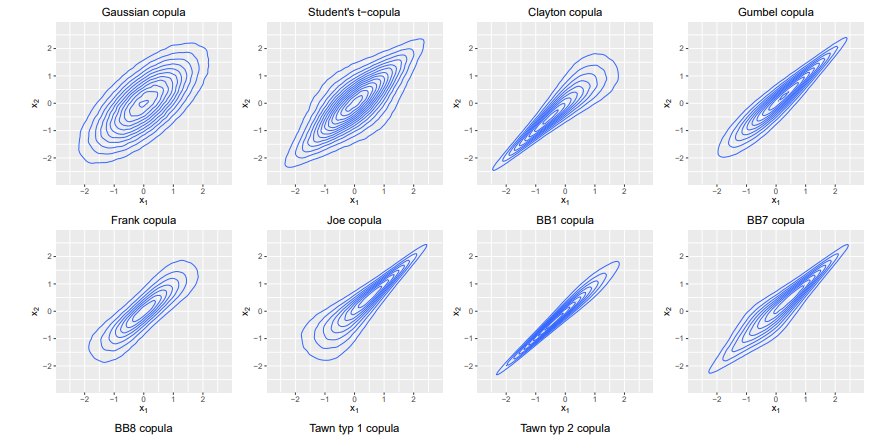
\includegraphics[scale=0.5]{taildep.png}
\label{fig:fig1}
\end{figure}

\end{frame}
%\begin{frame}[label=frame3d]
%	\frametitle{Worst Case Copula-CVaR}
	
%	\begin{itemize}
%		\justifying
%		
%		\item 	Theorem 1 of \textcolor{blue}{Zhu and Fukushima}, \textcolor{blue}{2009} states that for each
%		fixed $\mathbf{w}\in \mathcal{W}$ the $WCVaR_{\beta }\left( \mathbf{w}%
%		\right) $ with respect to the set $\mathcal{C}$ is represented by
%		
%	\end{itemize}
%		\begin{eqnarray}
%		WCVaR_{\beta }\left( \mathbf{w}\right) &=&\underset{}{\underset{\alpha \in
%				\mathbb{R}
%			}{\min }~\underset{\pi \in \Pi }{\max }}~H_{\beta }\left( \mathbf{w},\alpha
%		,\pi \right)  \notag \\
%		&=&\underset{}{\underset{\alpha \in
%				\mathbb{R}
%			}{\min }~\underset{\pi \in \Pi }{\max }}\sum_{i=1}^{d}\pi _{i}H_{\beta
%		}^{i}\left( \mathbf{w},\alpha \right) .  \label{31}
%		\end{eqnarray}%
		
%		\begin{itemize}
%			
%				
%%			\item Minimizing the
%%			worst-case Copula-CVaR over $\mathbf{w}\in \mathcal{W}$ can be defined as
%%			the following optimization problem:%
%%			\begin{equation}
%%			\underset{\mathbf{w}\in \mathcal{W}}{\min }WCVaR_{\beta }\left( \mathbf{w}%
%%			\right) =\underset{}{\underset{\mathbf{w}\in \mathcal{W}}{\min }~\underset{%
%%					\alpha \in
%%					\mathbb{R}
%%				}{\min }~\underset{\pi \in \Pi }{\sup }}~H_{\beta }\left( \mathbf{w},\alpha
%%			,\pi \right) .  \label{32}
%%			\end{equation}%
%			
%					
%	\end{itemize}
	

%\end{frame}

\begin{frame}[label=frame3e]
	\frametitle{Worst Case Copula-CVaR}
	
	\begin{itemize}
		\justifying
		\setlength{\parskip}{15pt}
		\setbeamercovered{transparent}
		
%		\begin{equation}
%		H_{\beta }^{i}\left( \mathbf{w},\alpha \right) =\alpha +\frac{1}{1-\beta }
%		\int_{\mathbf{u}\in \left[ 0,1\right] ^{n}}\left( \widetilde{h}\left( \mathbf{w,u}
%		\right) -\alpha \right) ^{+}c_{i}\left( \mathbf{u}\right) d\mathbf{u}. \label{30}
%		\end{equation}%
		
		\item By using the approach of \textcolor{blue}{Rockafellar and Uryasev} (\textcolor{blue}{2000}), the integral in 
		\begin{eqnarray*}
			H_{\beta }\left( \mathbf{w},\alpha ,\pi \right) &=&\alpha +\frac{1}{1-\beta }
			\int_{\mathbf{u}\in \left[ 0,1\right] ^{n}}\left( \widetilde{h}\left( \mathbf{w,u}
			\right) -\alpha \right) ^{+}\sum_{i=1}^{d}\pi _{i}c_{i}\left( \mathbf{u}
			\right) d\mathbf{u}\\
			&=&\sum_{i=1}^{d}\pi _{i}H_{\beta }^{i}\left( \mathbf{w},\alpha \right) ,
		\end{eqnarray*}
	is approximated by sample realizations from the copulas $%
		C_{i}\left( \cdot \right) \in \mathcal{C}$, by using as inputs the filtered
		uniform margins. 
		
		\item If the sampling generates a collection of values $\left(
		\mathbf{u}_{i}^{[1]},\mathbf{u}_{i}^{[2]},\ldots,\mathbf{u}_{i}^{[J]}\right) $,
		where $\mathbf{u}_{i}^{[j]}$ and $S^{i}$ are the $j$-th sample drawn from
		copula $C_{i}\left( \cdot \right) $, we can approximate $H_{\beta }^{i}\left( \mathbf{w},\alpha
		\right) $ by
		\begin{equation}
		\widetilde{H}_{\beta }^{i}\left( \mathbf{w},\alpha \right) =\alpha +\frac{1}{%
			\left( 1-\beta \right) S^{i}}\sum_{j=1}^{S^{i}}\left( \widetilde{h}(\mathbf{w},\mathbf{u}%
		_{i}^{[j]})-\alpha \right) ^{+},i=1,\ldots,d.
		\end{equation}%
		
				
	\end{itemize}
	
	
\end{frame}

\begin{frame}[label=frame3f]
	\frametitle{Optimization Problem}
	
	\begin{itemize}
		\setlength{\parskip}{15pt}
		\setbeamercovered{transparent}
		\justifying
		
		\item Assuming that the allowable set $\mathcal{W}$ is convex and the loss
		function $\widetilde{h}\left( \mathbf{w,u}\right) $ is linear with respect to $\mathbf{w}$, then optimization problem
%		\begin{equation}
%		\underset{\mathbf{w}\in \mathcal{W},\alpha \in
%			\mathbb{R}
%		}{\min }\widetilde{H}_{\beta }\left( \mathbf{w},\alpha \right) .
%		\end{equation}%
		reduces to the following LP problem:%
	\begin{alignat}{3}
	& \underset{\mathbf{w}\in
		\mathbb{R}^{n},v\in
		\mathbb{R}^{m},\alpha \in
		\mathbb{R}}{\text{minimize}}
	& & \alpha +\frac{1}{\left( 1-\beta \right)  S^{i}}\sum_{i=1}^{S^{i}}v_{i}
	\\ 
	& \text{subject to} 
	& & \mathbf{w}\in \mathcal{W},\\
	&&& v_{i}^{\left[ j\right] }\geq \widetilde{h}(\mathbf{w},\mathbf{u}_{i}^{[j]})-\alpha , \\
	&&&v_{i}^{\left[ j\right] }\geq 0, \; j = 1, \ldots, J; \ i = 1, \ldots, d,
	\end{alignat}
	where $v_{i}$, $i = 1, \ldots, d$, are auxiliary indicator (dummy) variables and $m=\sum_{i=1}^{d}S^{i}$. 

	\item By solving the LP problem, we find the optimal
	decision vector, $\mathbf{w}^{\ast }$, and at ``one shot'' the optimal $VaR$, $
		\alpha ^{\ast }$, and the optimal $CVaR$, \footnotesize $\widetilde{H}_{\beta }\left(	\mathbf{w}=\mathbf{w}^{\ast },\alpha =\alpha ^{\ast }\right) $.
		
	
		\end{itemize}
\end{frame}


\section{Data}

\begin{frame}[label=frame2b]
\frametitle{Data}
\begin{itemize}

\setlength{\parskip}{15pt}
\setbeamercovered{transparent}
\justifying
	
	\item 	\textbf{Sources}: Adjusted closing prices for each stock.
	
%	\begin{itemize}
%		\item Cumulative total return index for each stock.
%	\end{itemize}
	\item \textbf{Universe}: All shares that belongs to the S\&P 500 market index.  
	%\begin{itemize}
	%	\setlength\itemsep{1em}
	\item \textbf{Period}: July 2nd, 1990 to December 31st, 2015.
	\item \textbf{Total}: 1100 stocks over a 6426-day sample period.
	
\end{itemize}

\end{frame}

\section{Methodology}

\begin{frame}[label=frame4h]
	\frametitle{Methodology}
	
	\begin{itemize}
		\setlength{\parskip}{15pt}
		\setbeamercovered{transparent}
		\justifying
		
		\item<1> Our optimization strategy adopts a sliding window of calibration of four years of daily data.
		
		\item<1> We rebalance our portfolio every six months.
		
		\item<2> We select, among all listed stocks in each formation period, a set of 50 stocks based on the ranked sum of absolute spreads (the 25 largest and the 25 smallest) between the normalized daily closing prices deviations of the
		S\&P 500 index and all shares.
		
		\item<2> We use day $1$ to $T$, where $T$ is the sliding window, to estimate the parameters of all models and determine the portfolio weights for day $T+1$ and then repeat the process including the latest observation and removing the oldest until we reach the end of the time series. 

		\end{itemize}
	
\end{frame}

\subsection{Strategies Under Analysis}

\subsubsection{Worst Case Copula-CVaR Portfolio Optimization}
\begin{frame}[label=frame5]
\frametitle{Worst Case Copula-CVaR Portfolio Optimization}

\begin{enumerate}
	\setcounter{enumi}{0}
	\setlength{\parskip}{15pt}
	\setbeamercovered{transparent}
\justifying
\item We fit an AR(1)-GARCH(1,1) model with skew $t$-distributed innovations to each univariate time series.

\item Using the estimated parametric model, we construct the standardized
residuals vectors given, for each $i=1,\ldots,50$ and $t=1,\ldots,L-T-1$, where $L$ is the data set sample period, by
\begin{equation*}
\frac{\widehat{\varepsilon }_{i,t}}{\widehat{\sigma }_{i,t}}.
\end{equation*}%
The standardized residuals vectors are then converted to pseudo-uniform
observations $z_{i,t}=\frac{n}{n+1}F_{i}\left( \widehat{\varepsilon }%
_{i,t}\right) $, where $F_{i}$ is their empirical distribution function.

 
 \end{enumerate}

\end{frame}

\begin{frame}[label=frame5b]
	\frametitle{Worst Case Copula-CVaR Portfolio Optimization}
	
	\setlength{\parskip}{15pt}
	\setbeamercovered{transparent}
	
	\begin{enumerate}
		\setcounter{enumi}{2}
		\justifying
		\item Estimate the copula model, i.e., fits the multivariate Clayton-Frank-Gumbel
		(CFG) Mixture Copula to data that has been transformed to $[0,1]$ margins by
		\begin{equation}
		C^{CFG}( \Theta ,\mathbf{u}) =\pi _{1}C^{C}( \theta _{1},\mathbf{u}) +\pi
		_{2}C^{F}( \theta_{2},\mathbf{u}) +(1-\pi _{1}-\pi _{2}) C^{G}( \theta _{3},%
		\mathbf{u})
		\end{equation}
		where $\Theta=\left(\alpha,\beta,\delta\right)^{\top }$ are the Clayton,
		Frank and Gumbel copula parameters, respectively, and $\pi_{1}$, $\pi_{2}
		\in [0,1]$. 
		\setlength{\parskip}{5pt}
		\begin{itemize}
%			\item The estimates are obtained by the minimization of the negative
%			log-likelihood consisting of the weighted densities of the Clayton, Frank
%			and Gumbel copulas.
			\item Probability density function for multivariate Archimedean copula is computed as described in \textcolor{blue}{McNeil and Neshelova} (\textcolor{blue}{2009}).
		\end{itemize} 
		
		\setlength{\parskip}{15pt}

		\item Use the dependence structure determined by the estimated copula for generating $J $ scenarios. To simulate data from the three Archimedean copulas we use the sampling algorithms provided in \textcolor{blue}{Melchiori} (\textcolor{blue}{2006}).
		
	\item Compute $t$-quantiles for these Monte Carlo draws. 
		
		\end{enumerate}
	
\end{frame}

\begin{frame}[label=frame5c]
	\frametitle{Worst Case Copula-CVaR Portfolio Optimization}
	
	\begin{enumerate}
		\setcounter{enumi}{5}
		\justifying
		\setlength{\parskip}{15pt}
		\setbeamercovered{transparent}
		
		\item Compute the standard deviation $%
		\widehat{\sigma }_{i,t}$ using the estimated GARCH model.
		
		\item Determine the simulated daily asset log-returns, i.e., determine the simulated daily log-returns as $r_{i,t}^{sim}=\widehat{\mu }_{t}+\widehat{\sigma }_{i,t}z_{i,t}$.
		
		\item Finally, use the simulated data as inputs when optimizing portfolio weights by minimizing CVaR for a given confidence level and a given minimum expected return.
		
	\end{enumerate}

\end{frame}

\begin{frame}[label=frame5d]
\frametitle{Worst Case Copula-CVaR Portfolio Optimization}

\setlength{\parskip}{15pt}
\setbeamercovered{transparent}

\begin{itemize}
\justifying
\setlength{\parskip}{15pt}
\setbeamercovered{transparent}

	\item For each of the three copulas, we run 1000 return scenarios from the
	estimated multivariate CFG Mixture Copula model.
	
	\item The weights are recalibrated at a daily, weekly and monthly basis. We assume
	that the feasible set $\mathcal{W}$ attends the following linear constraints:
	
	\setlength{\parskip}{2pt}
	
	\begin{itemize}
		
		\item The sum of the weights should be 1, i.e., $\mathbf{w}^{\top }\mathbf{1=}1$; 
		
		\item No short-selling: $\mathbf{w\geq }0$;
		
		\item The expected return should be bound below by an arbitrary value $\overline{r}$, i.e., $\mathbf{w}^{^{\top }}\mathbb{E}\left( \mathbf{r}%
		_{p,t+1}\right) \mathbf{\geq }\overline{r}$, where $\overline{r}$ represents the target mean return;
		
		\end{itemize}
	
	\setlength{\parskip}{15pt}
	
	\item The confidence level $\beta $ is set at $\beta =0.95$.
	
\end{itemize}

\end{frame}


\begin{frame}[label=frame7]
\frametitle{Benchmarks}

\begin{itemize}
\justifying
\setlength{\parskip}{15pt}
\setbeamercovered{transparent}

\item Gaussian Copula Portfolio.

\item Equally-weighted portfolio $w_{i} = 1/N$, i.e. $\mathbf{w=}\left( \frac{1}{N},\ldots,\frac{1}{N}\right) {^{\top }}$ for
any reba-lancing date $t$.

\item S\&P 500 index as a proxy for market return.

\item More benchmarks (to come): extended (robust) versions of the classic Markowitz model, shrinkage portfolios, VaR and CVaR optimal portfolios under multivariate normality, etc. 

%control the downside risk of the portfolio returns.

%Usually the objective is to find the optimal risk-return trade-off.

\end{itemize}

\end{frame}

%\begin{frame}[label=frame7]
%\frametitle{Simulating from a Gaussian Copula}
%
%\setlength{\parskip}{15pt}
%\setbeamercovered{transparent}
%
%From Sklar's theorem the Gauss copula is given by \begin{equation}C_{p}\left (u_{1} , . . . ,u_{d}\right ) =\mathbf{\Phi }_{p}\left (\Phi ^{ -1}(u_{1}) , . . . ,\Phi ^{ -1}(u_{d})\right ) ,
%\end{equation}where $\Phi $ denotes the standard normal distribution function, and $\mathbf{\Phi }_{p}$ denotes the multivariate standard normal distribution function with correlation matrix $P .$
%
%\begin{itemize}
%	\justifying
%	\item Repeat the following steps $n$ times.
%	
%	\begin{itemize}
%	\item Perform a Cholesky decomposition of $P$, and set $A$ as the resulting lower triangular matrix.
%	
%	\item Generate a vector $Z =\left (Z_{1} , . . . ,Z_{d}\right )^{ \prime ^{\,}}$of independent standard normal variables.
%	
%	\item Set $X =AZ$.
%	
%	\item Return $U =\left (\Phi (X_{1})\right . , . . . ,\Phi ^{\,}(X_{d}))^{ \prime ^{\,}}$.
%	\end{itemize}
%	
%\end{itemize}
%
%\end{frame}

\section{Performance Measures}

\begin{frame}
\frametitle{Performance Measures}

\begin{itemize}
	
	\setlength{\parskip}{15pt}
	\setbeamercovered{transparent}

%\begin{equation}
%\widehat{\mu }_{p}=\frac{1}{L-T}\sum\nolimits_{t=T+1}^{L-1}\widehat{r}_{p,t},
%\end{equation}
% $t=T+1,...,L-1$, where 
%\begin{equation}
%\widehat{r}_{p,t}=\mathbf{w}_{t-1}^{^{\top }}\mathbf{r}_{p,t}-r_{f,t}\text{,}
%\end{equation}%

%\begin{equation}
%\widehat{\sigma }_{p}=\sqrt{\frac{1}{L-T-2}\sum\nolimits_{t=T}^{L-1}\left(
%	w_{t}r_{p,t+1}-\widehat{\mu }_{p}\right) ^{2}},
%\end{equation}%

\item Portfolio mean excess return and standard deviation;

\item Sharpe and Sortino Ratios;

\item Maximum drawdown;

\item Turnover.

\setlength{\parskip}{0pt}

\begin{itemize}
%	\item Turnover measures the amount of trading required to implement a particular portfolio strategy and can be interpreted as the average fraction	of wealth traded in each period.
	\item The higher the turnover, the higher the transaction cost that the portfolio incurs at each rebalancing day.
\end{itemize}

\setlength{\parskip}{15pt}

\item Break-even transaction cost:  level of transaction costs that makes the investor indifferent between the dynamic and the static strategies.
%, i.e., the maximum transaction cost that can be imposed before making the strategies less desirable than the buy-and-hold strategy.

% (\textcolor{blue}{Bessembinder and Chan}, \textcolor{blue}{1995}) is the level of transaction costs leading to zero
%net profits, i.e., the maximum transaction cost that can be imposed before
%making the strategies less desirable than the buy-and-hold strategy. Following \textcolor{blue}{Santos and Tessari}, \textcolor{blue}{2012} we consider the average net
%returns on transaction costs, $\widehat{\mu }_{TC}$, given by
%\setlength{\parskip}{0pt}
%
%\begin{itemize}
%	\item Portfolios that achieve a higher break-even cost are preferable, since the level required to make these portfolios non-profitable are higher.
%\end{itemize}

%\item We define the portfolio turnover from time $t$ to time $t+1$ as the sum of
%the absolute changes in the $N$ risky asset weights, i.e., in the optimal
%values of the investment fractions:

%\begin{equation}
%Turnover=\frac{1}{L-T-1}\sum\nolimits_{t=T}^{L-1}\sum\nolimits_{j=1}^{N}%
%\left( \left\vert w_{j,t+}-w_{j,t+1}\right\vert \right) ,
%\end{equation}%
%where $w_{j,t+}^{{}}$ is the actual weight in asset $j$ before rebalancing
%at time $t+1$, and $w_{j,t+1}$ is the optimal weight in asset $j$ at time $%
%t+1$. 

\end{itemize}

\end{frame}

%\begin{frame}
%	\frametitle{Performance Measures}
%	
%	\begin{enumerate}
%		\setcounter{enumi}{2}
		
%		\begin{equation}
%		SR=\frac{\widehat{\mu }_{p}}{\widehat{\sigma }_{p}}.
%		\end{equation}
		
%		\item The maximum drawdown on the interval $[0,T]$ is defined as
%		\begin{equation}
%		MaxDD\left( \mathbf{w}\right) =\underset{0\leq \tau \leq t}{\max }\left\{
%		D\left( \mathbf{w,}t\right) \right\} .
%		\end{equation}
%		In other words, the maximum drawdown over a period is the maximum loss from
%		worst peak to a trough of a portfolio drop from the start to the end of the
%		period.
		
%		\end{enumerate}
%
%\end{frame}

%\begin{frame}
%	\frametitle{Performance Measures}
%	
%\setlength{\parskip}{15pt}
%\setbeamercovered{transparent}
%	
%	\begin{enumerate}
%		\setcounter{enumi}{4}
		
%		\item The Sortino's ratio (\textcolor{blue}{Sortino}, \textcolor{blue}{1994}) is the ratio of the mean excess	return to the standard deviation of negative asset returns, i.e.,
%		
%		\begin{equation}
%		SoR=\frac{\widehat{\mu }_{p}}{\widehat{\sigma }_{p,n}},
%		\end{equation}%
%		where
%		
%		\begin{equation}
%		\widehat{\sigma }_{p,n}=\sqrt{\frac{1}{L-T-1}\sum\nolimits_{t=T}^{L-1}\left(
%			\min \left( 0,\mathbf{w}_{t}^{^{\top }}\mathbf{r}_{t+1}-\mathbf{r}%
%			_{MAR}\right) \right) ^{2}},
%		\end{equation}%
%		where $\mathbf{r}_{MAR}$ is the value of a minimal acceptable return (MAR),
%		usually zero or the risk-free rate.
		
%	\end{enumerate}
%		
%\end{frame}

%\begin{frame}
%	\frametitle{Performance Measures}
%	
%\setlength{\parskip}{15pt}
%\setbeamercovered{transparent}
%	
%	\begin{enumerate}
%		\setcounter{enumi}{5}
		
%		\item We define the portfolio turnover from time $t$ to time $t+1$ as the sum of
%		the absolute changes in the $N$ risky asset weights, i.e., in the optimal
%		values of the investment fractions:
%		
%		\begin{equation}
%		Turnover=\frac{1}{L-T-1}\sum\nolimits_{t=T}^{L-1}\sum\nolimits_{j=1}^{N}%
%		\left( \left\vert w_{j,t+}-w_{j,t+1}\right\vert \right) ,
%		\end{equation}%
%		where $w_{j,t+}^{{}}$ is the actual weight in asset $j$ before rebalancing
%		at time $t+1$, and $w_{j,t+1}$ is the optimal weight in asset $j$ at time $%
%		t+1$. 
%			
%		\end{enumerate}
%		
%		\begin{itemize}
%		
%		\end{itemize}
%		
%		
%\end{frame}

\begin{frame}
\frametitle{Performance Measures}

\setlength{\parskip}{15pt}
\setbeamercovered{transparent}

%	\begin{equation}
%	\widehat{\mu }_{TC}=\frac{1}{L-T}\sum\nolimits_{t=T}^{L-1}\left[ \left( 1+%
%	\mathbf{w}_{t}^{^{\top }}\mathbf{r}_{t+1}\right) \left(
%	1-c\sum\nolimits_{j=1}^{N}\left( \left\vert w_{j,t+1}-w_{j,t+}\right\vert
%	\right) \right) -1\right] ,
%	\end{equation}%
%	where $c$ is\ called breakeven cost when we solve $\widehat{\mu }_{TC}=0.$
	
	\begin{itemize}
	
	\item Capital requirement loss function (CR)
	
	\begin{itemize}
		\item Regulatory loss function to evaluate VaR forecasts
	\end{itemize}
	
	\begin{equation}CR_{t} =\max \left [\left (\genfrac{(}{)}{}{}{3 +\delta }{60}\sum _{i =0}^{59}VaR_{\beta  ,t -i}\right ) ,VaR_{\beta  ,t}\right ] ,
	\end{equation}where $\delta $ is a multiplicative factor that depends on the number of violations of the VaR in the previous 250 trading days.
	
	\begin{itemize}
		\item To mitigate data-snooping problems we apply a test for superior predictive ability (SPA) proposed by \textcolor{blue}{Hansen} (\textcolor{blue}{2005}) to determine which model significantly minimizes the expected loss function. 
	\end{itemize}

\end{itemize}
	
\end{frame}

\section{Empirical Results}

\begin{frame}
	\frametitle{Empirical Results}
	
	\definecolor{corn}{rgb}{0.98, 0.93, 0.36}
	\definecolor{celadon}{rgb}{0.67, 0.88, 0.69}
	
	\begin{threeparttable}[H]
		\caption{\footnotesize Excess returns of Worst Case Copula-CVaR (WCCVaR), Gaussian Copula-CVaR (GCCVaR) and Equal Weights portfolios without a minimum expected return constraint}
		\label{tab:tabletwo}\centering
		\tiny \
		\begin{tabularx}{\textwidth}{@{\extracolsep{\fill}}lcccc@{}}
			\toprule & \textbf{WCCVaR} & \textbf{GCCVaR} & \textbf{1/N} & \textbf{S\&P 500%
			} \\
			\midrule[\heavyrulewidth] \textit{Daily Rebalancing} &  &  &  &  \\
			\midrule[\heavyrulewidth] Mean Return (\%) & \cellcolor{corn} 11.29 & 10.59 & 10.52 & 6.61
			\\
			Standard Deviation (\%) & 15.35 & \cellcolor{celadon} 15.05 & 23.86 & 19.01 \\
			Sharpe Ratio & \cellcolor{corn} 0.70 & 0.67 & 0.42 & 0.34 \\
			Sortino Ratio & 1.14 & 1.09 & 0.68 & 0.54 \\
			Turnover & 0.6868 & 0.6425 & 0.0001 &  \\
			Break-even (\%) & 0.0618 & 0.0622 & 275.09 &  \\
			MDD1 (\%) & -13.20 & \cellcolor{celadon} -12.89 & -18.00 & -13.20 \\
			MDD2 (\%) & \cellcolor{corn} -38.94 & -41.66 & -71.84 & -52.61 \\
			VaR$_{0.95}$ & \cellcolor{corn} 0.0091 & 0.0109 & 0.0209  & 0.0170 \\
			CVaR$_{0.95}$ & \cellcolor{corn} 0.0109 & 0.0135 & 0.0323 & 0.0283  \\
			CR$_{0.05} (\%)$ & \cellcolor{corn} $13.00^{***}$ & 15.63 & 29.71 & 23.91  \\
			\midrule[\heavyrulewidth] \textit{Weekly Rebalancing} &  &  &  &  \\
			\midrule[\heavyrulewidth] Mean Return (\%) & 10.57 & 10.04 & 10.52 & 6.61
			\\
			Standard Deviation (\%) & 15.48 & 15.21 & 23.86 & 19.01 \\
			Sharpe Ratio & 0.65 & 0.63 & 0.42 & 0.34 \\
			Sortino Ratio & 1.06 & 1.02 & 0.68 & 0.54 \\
			Turnover & 0.1535 & 0.1564 & 0.0001 &  \\
			Break-even (\%) & \cellcolor{corn} 0.2596 & \cellcolor{celadon} 0.2427 & 275.09 &  \\
			MDD1 (\%) & -12.59 & -10.39 & -18.00 & -13.20 \\
			MDD2 (\%) & -39.78 & -41.32 & -71.84 & -52.61 \\
			VaR$_{0.95}$ &  0.0091 & 0.0109 & 0.0209  & 0.0170 \\
			CVaR$_{0.95}$ & 0.0109 & 0.0135 & 0.0323 & 0.0283 \\
			CR$_{0.05}$ (\%) & \cellcolor{corn} $12.86^{***}$ & 15.57 & 29.71  & 23.91  \\
			\bottomrule &  &  &  &
		\end{tabularx}%
		\label{tab:table02}%
	\end{threeparttable}

	\end{frame}

\begin{frame}
	\frametitle{Empirical Results}
	
	\definecolor{corn}{rgb}{0.98, 0.93, 0.36}
	\definecolor{celadon}{rgb}{0.67, 0.88, 0.69}
	
	\begin{threeparttable}[H]
		\caption{Excess returns of Worst Case Copula-CVaR (WCCVaR), Gaussian Copula-CVaR (GCCVaR) and Equal Weights portfolios without a daily minimum expected return constraint}
		\label{tab:tabletwo}\centering
		\tiny \
		\begin{tabularx}{\textwidth}{@{\extracolsep{\fill}}lcccc@{}}
			\toprule & \textbf{WCCVaR} & \textbf{GCCVaR} & \textbf{1/N} & \textbf{S\&P 500%
			} \\
						\midrule[\heavyrulewidth] \textit{Monthly Rebalancing} &  &  &  &  \\
						\midrule[\heavyrulewidth] Mean Return (\%) & 9.22 & 9.42 & 10.52 & 6.61
						\\
						Standard Deviation (\%) & 15.69 & 15.55 & 23.86 & 19.01 \\
						Sharpe Ratio & 0.56 & 0.58 & 0.42 & 0.34 \\
						Sortino Ratio & 0.91 & 0.94 & 0.68 & 0.54 \\
						Turnover & 0.0447 & 0.0499 & 0.0001 &  \\
						Break-even (\%) & \cellcolor{corn} 0.7829 & \cellcolor{celadon} 0.7155 & 275.09 &  \\
						MDD1 (\%) & -13.21 & -13.22 & -18.00 & -13.20 \\
						MDD2 (\%) & -38.58 & -46.13 & -71.84 & -52.61 \\
						VaR$_{0.95}$ &  0.0091 & 0.0109 & 0.0209  & 0.0170 \\
							CVaR$_{0.95}$ & 0.0109 & 0.0134 & 0.0323 & 0.0283 \\
						CR$_{0.05}$ (\%) & \cellcolor{corn} $12.22^{***}$ & 14.67 & 29.71  & 23.91  \\
			\bottomrule &  &  &  &
		\end{tabularx}%
		\begin{tablenotes}
			\item \textit{Note:} \tiny Out-of-sample performance statistics between July 1994 and December 2015 (5414 observations). The rows labeled MDD1 and MDD2 compute the largest drawdown in terms of maximum percentage drop between two consecutive days and between two days within a period of maximum six months, respectively. Returns, standard deviation, Sharpe ratio and Sortino ratio are annualized.
			\item \scriptsize $^{\ast\ast\ast}$ , $^{\ast\ast}$, $^{\ast}$ significant at 1\%, 5\% and 10\% levels, respectively.
		\end{tablenotes}
		\label{tab:table02}%
	\end{threeparttable}
	
\end{frame}

\begin{frame}[label=frame10]
\frametitle{Cumulative Excess Returns}

\begin{figure}[htbp]
\centering
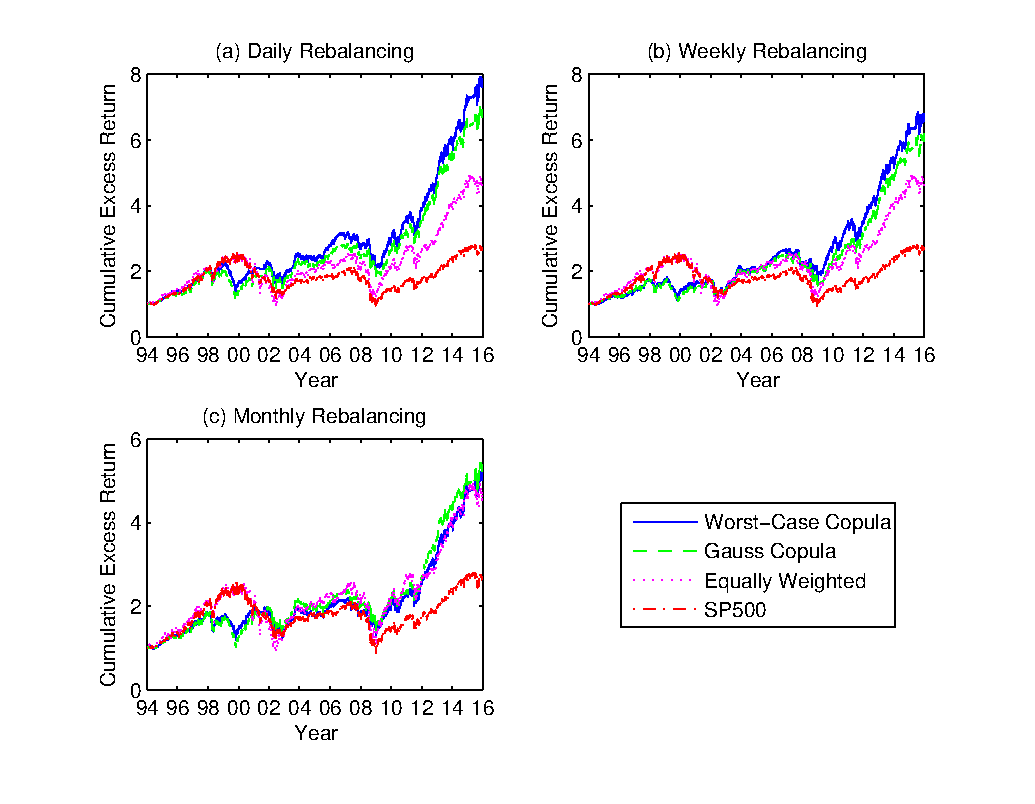
\includegraphics[scale=0.55]{fig1_nogrid.eps}
\caption{\scriptsize Cumulative excess returns of the portfolio strategies without daily target mean return }
\label{fig:fig01}
\end{figure}

\end{frame}

\begin{frame}[label=frame9d]
	\frametitle{Conclusions}
	
	\begin{itemize}
		\justifying
		\setlength{\parskip}{15pt}
		\setbeamercovered{transparent}
		
		\item By selecting a diversified set of assets over a long-term period we found that copula-based approaches offer better hedges against losses than the 1/N portfolio.
		
		\item The WCCVaR approach generates portfolios with better downside risk statistics for any rebalancing period and it is more profitable than the Gaussian Copula-CVaR for daily and weekly rebalancing. 
		
		\end{itemize}
	
\end{frame}
		
		\begin{frame}[label=frame9e]
		\frametitle{Extensions}
		
	
	\setlength{\parskip}{15pt}
		
		\begin{itemize}
			\setlength{\parskip}{5pt}
			\item Machine Learning and AI-based solutions. 
			%(Man + Machine and NOT Man vs Machine) 
			\begin{itemize}
				\item Optimizer Search with Reinforcement Learning.
				\begin{itemize}
					\item Stability issues.
					\item Finding the portfolio with the highest downside risk-adjusted performance (Sortino ratio, Omega, Kappa).
				\end{itemize}
				% maximize Sharpe ratio
			\end{itemize}
		
		\end{itemize}
	
	%funcao = @optPort_sharpe; %fitness function
		
		\end{frame}


\begin{frame}

\centering
\Large{Thanks! Any questions?}

\end{frame}

\end{document}


